%%%%%%%%%%%%%%%%%%%%%%%%%%%%%%%%%%%%%%%%%%%%%%%%%%%%%%%%%%%%%%%%%%%%%%%%%%%%%%%

\section*{\large Exercício 7 - Singularity Multifractal Spectra (SMS), também conhecido como MDFA}
\addcontentsline{toc}{chapter}{\protect\numberline{}\large Exercício 7}%

Os resultado das análises das famílias de sinais deste exercício se encontram na pasta \textbf{Exercise7} organizados nas pastas \textbf{7.2} e \textbf{7.3}.

\subsection*{7.1}
\addcontentsline{toc}{section}{\protect\numberline{} 7.1}%

O algoritmo foi alterado e se encontra na pasta \textbf{statistical\_analysis\_codes}.

\subsection*{7.2}
\addcontentsline{toc}{section}{\protect\numberline{} 7.2}%

Os códigos desta questão se encontram separados pelos grupos da tabela \textit{Dataset\_signal}. Os resultados a seguir são para o grupo noise com $n$ = 8192, e estão presentes na pasta \textbf{grupo\_noise} dentro da pasta referente a este exercício - \textbf{7.2}.

\begin{figure}[ht!]
	%\caption{Série e histogramas.}
	\vspace{0mm}	% acrescentar o espaçamento vertical apropriado entre o título e a borda superior da figura
	\begin{center}
		\resizebox{13cm}{!}{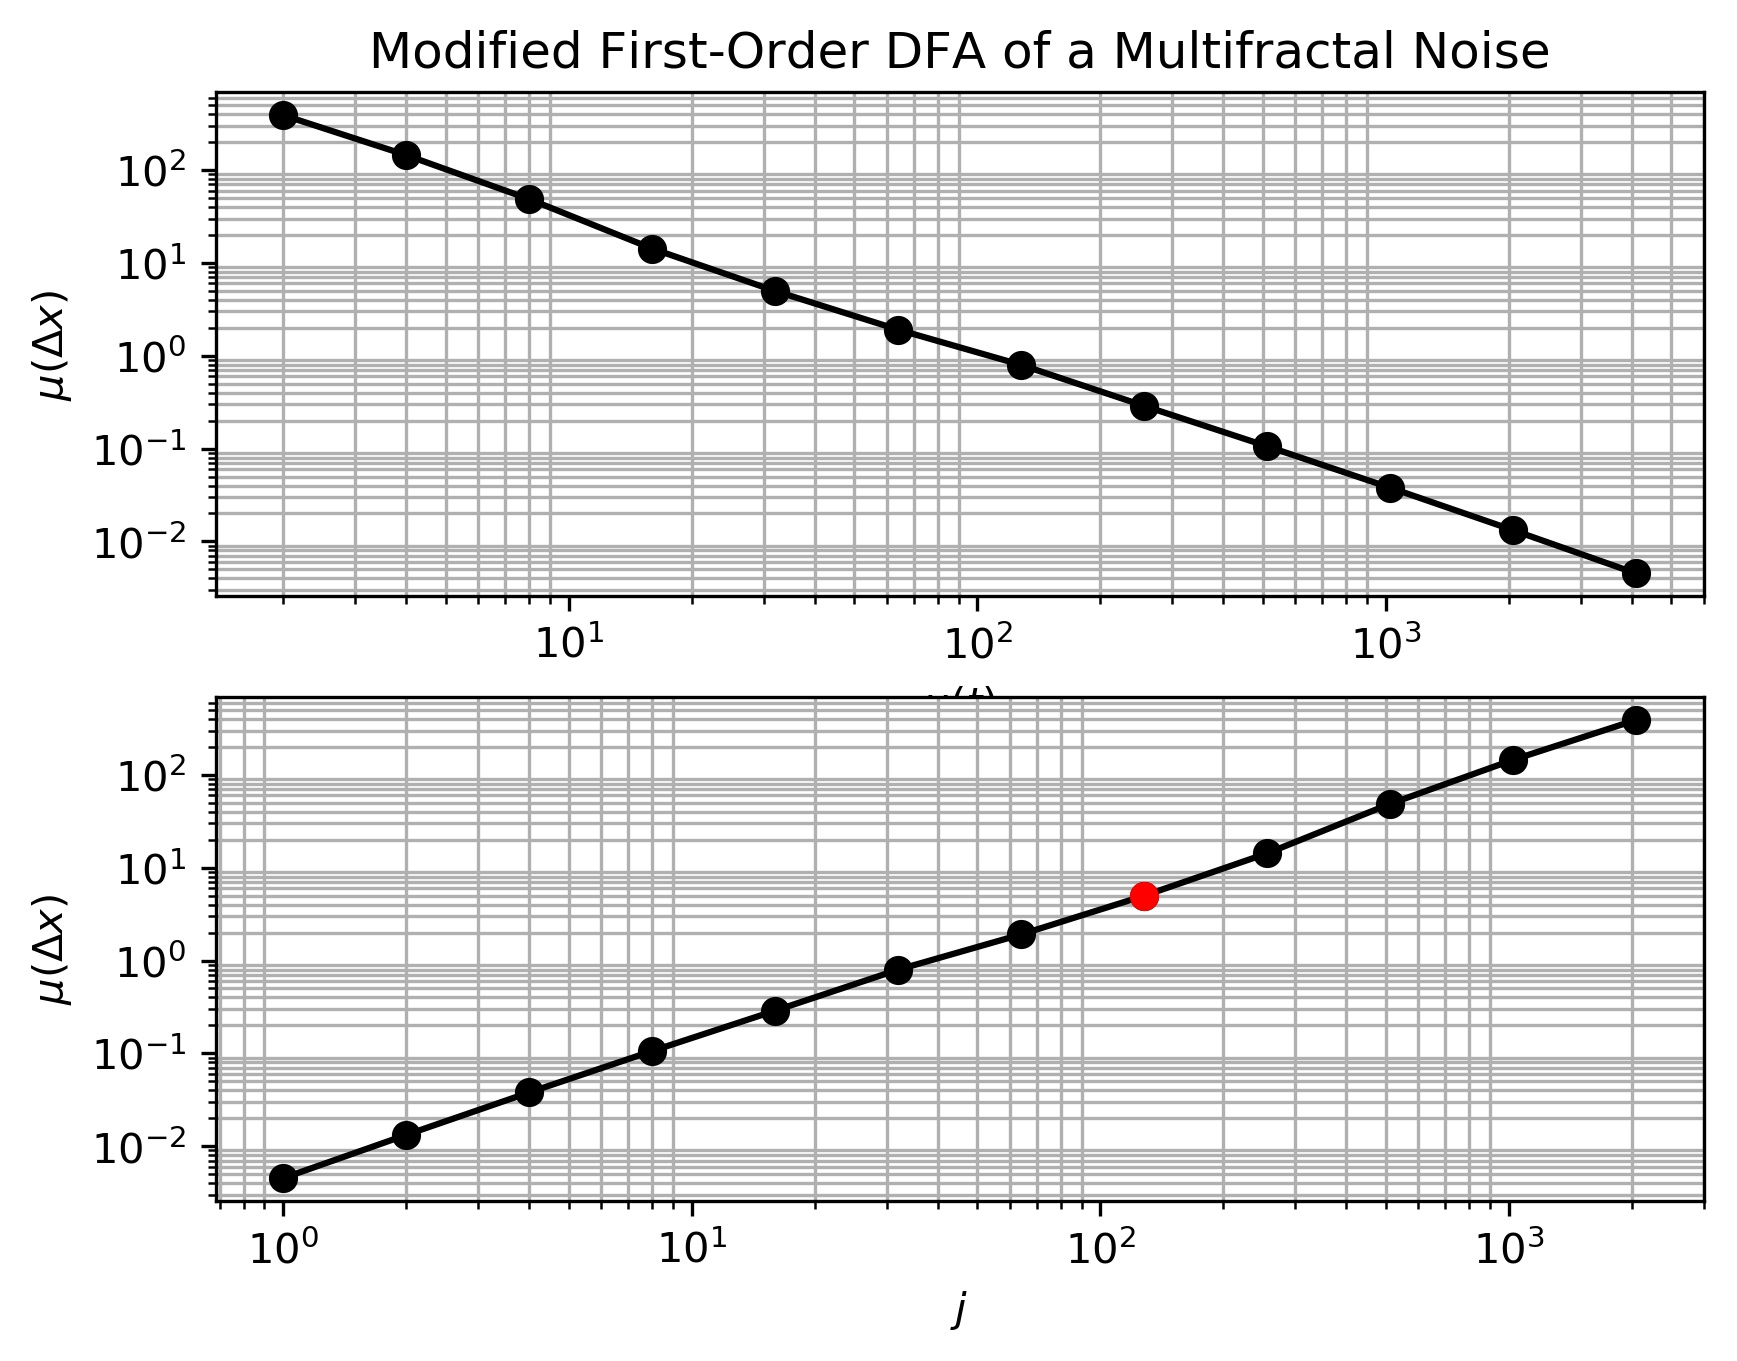
\includegraphics{Figuras/ex7/7_2/Exercicio7_2_grupo_noise_n_8192_mfdfa_1.jpg}}		
	\end{center}
	\vspace{-2mm}	% acrescentar o espaçamento vertical apropriado entre a borda inferior da figura e a legenda ou a fonte quando não há legenda (o valor pode ser negativo para subir)
	\legenda{Figura 7.2.1:. Topo: média da função de flutuação x tempo medido nas diferentes escalas; abaixo: média da função de flutuação x escala. Ambos os plots em log-log. Grupo noise com $n$ = 8192.}	% legenda - para deixar sem legenda usar comando \legenda{} (nunca deve-se comentar o comando \legenda)
	\label{ex6_fig1}
	%\FONTE{}	% fonte consultada (elemento obrigatório, mesmo que seja produção do próprio autor)
\end{figure}

\begin{figure}[ht!]
	%\caption{Série e histogramas.}
	\vspace{0mm}	% acrescentar o espaçamento vertical apropriado entre o título e a borda superior da figura
	\begin{center}
		\resizebox{13cm}{!}{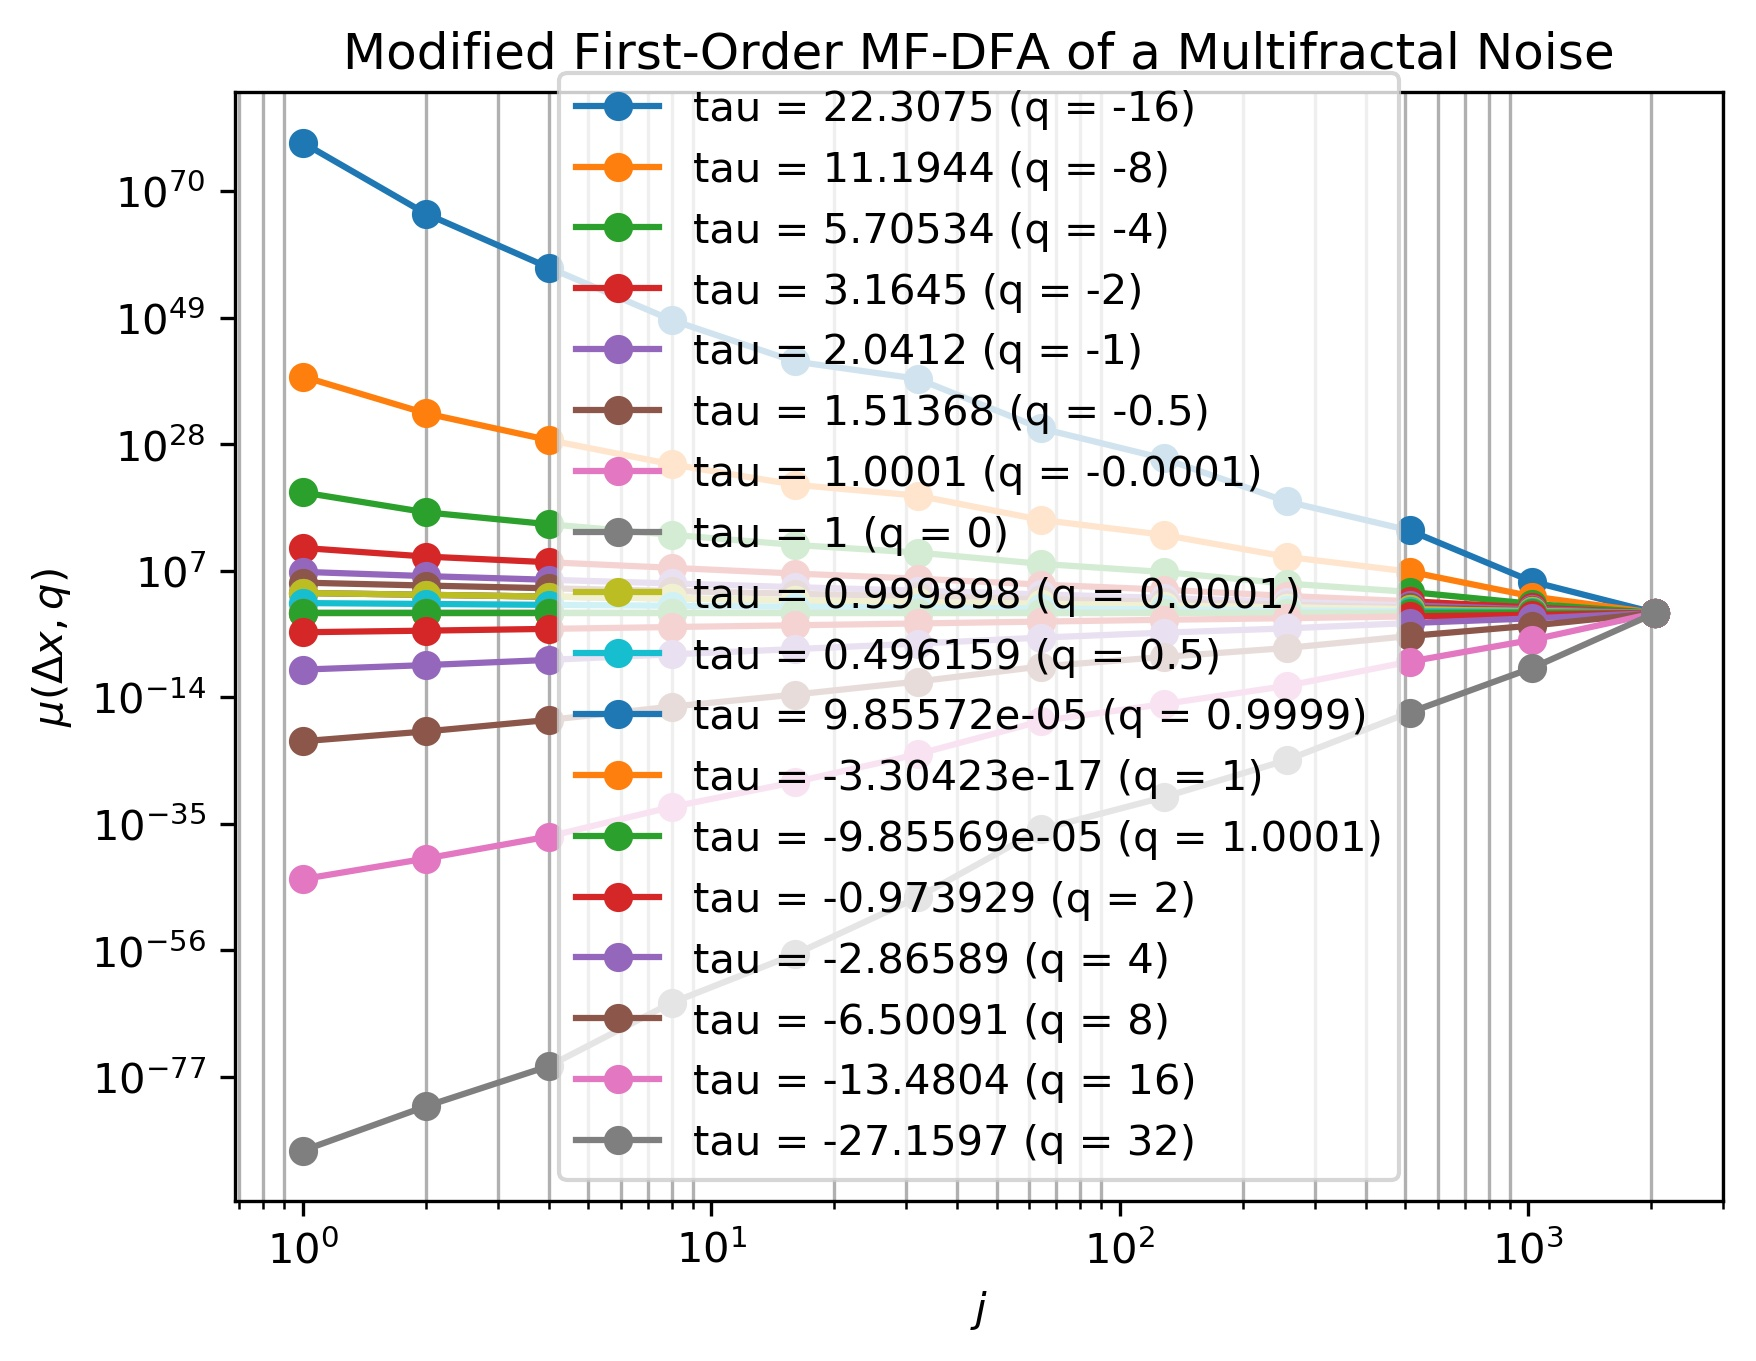
\includegraphics{Figuras/ex7/7_2/Exercicio7_2_grupo_noise_n_8192_mfdfa_2.jpg}}		
	\end{center}
	\vspace{-2mm}	% acrescentar o espaçamento vertical apropriado entre a borda inferior da figura e a legenda ou a fonte quando não há legenda (o valor pode ser negativo para subir)
	\legenda{Figura 7.2.2: Função de flutuação x escala em plot log-log para diferentes valores do expoente $q$. Grupo noise com $n$ = 8192.}	% legenda - para deixar sem legenda usar comando \legenda{} (nunca deve-se comentar o comando \legenda)
	\label{ex6_fig1}
	%\FONTE{}	% fonte consultada (elemento obrigatório, mesmo que seja produção do próprio autor)
\end{figure}

\begin{figure}[ht!]
	%\caption{Série e histogramas.}
	\vspace{0mm}	% acrescentar o espaçamento vertical apropriado entre o título e a borda superior da figura
	\begin{center}
		\resizebox{13cm}{!}{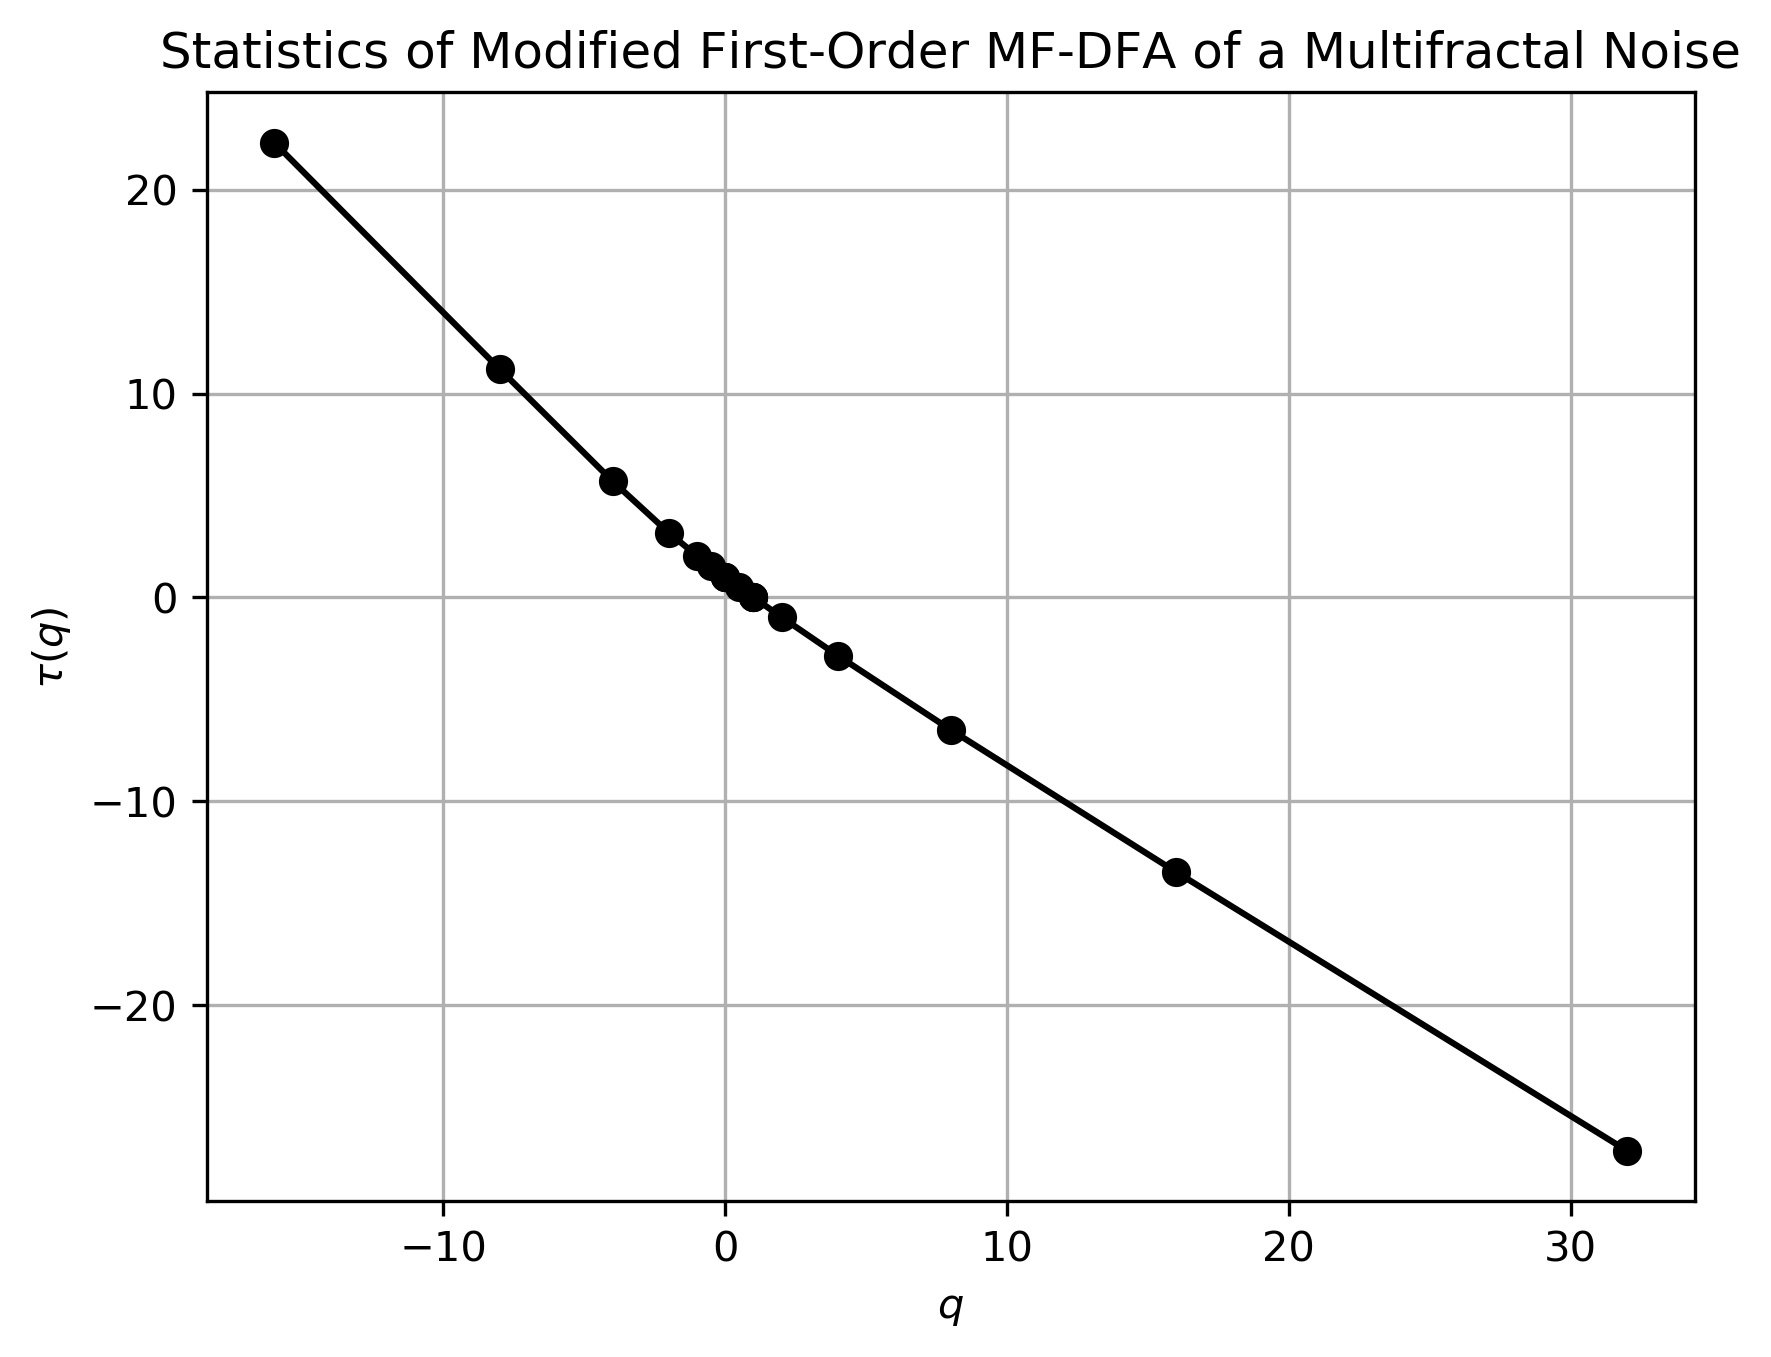
\includegraphics{Figuras/ex7/7_2/Exercicio7_2_grupo_noise_n_8192_mfdfa_3.jpg}}		
	\end{center}
	\vspace{-2mm}	% acrescentar o espaçamento vertical apropriado entre a borda inferior da figura e a legenda ou a fonte quando não há legenda (o valor pode ser negativo para subir)
	\legenda{Figura 7.2.3: Dependência de $\tau(q)$ com $q$ do grupo noise para $n$ = 8192.}	% legenda - para deixar sem legenda usar comando \legenda{} (nunca deve-se comentar o comando \legenda)
	\label{ex6_fig1}
	%\FONTE{}	% fonte consultada (elemento obrigatório, mesmo que seja produção do próprio autor)
\end{figure}
\clearpage
\begin{figure}[ht!]
	%\caption{Série e histogramas.}
	\vspace{0mm}	% acrescentar o espaçamento vertical apropriado entre o título e a borda superior da figura
	\begin{center}
		\resizebox{13cm}{!}{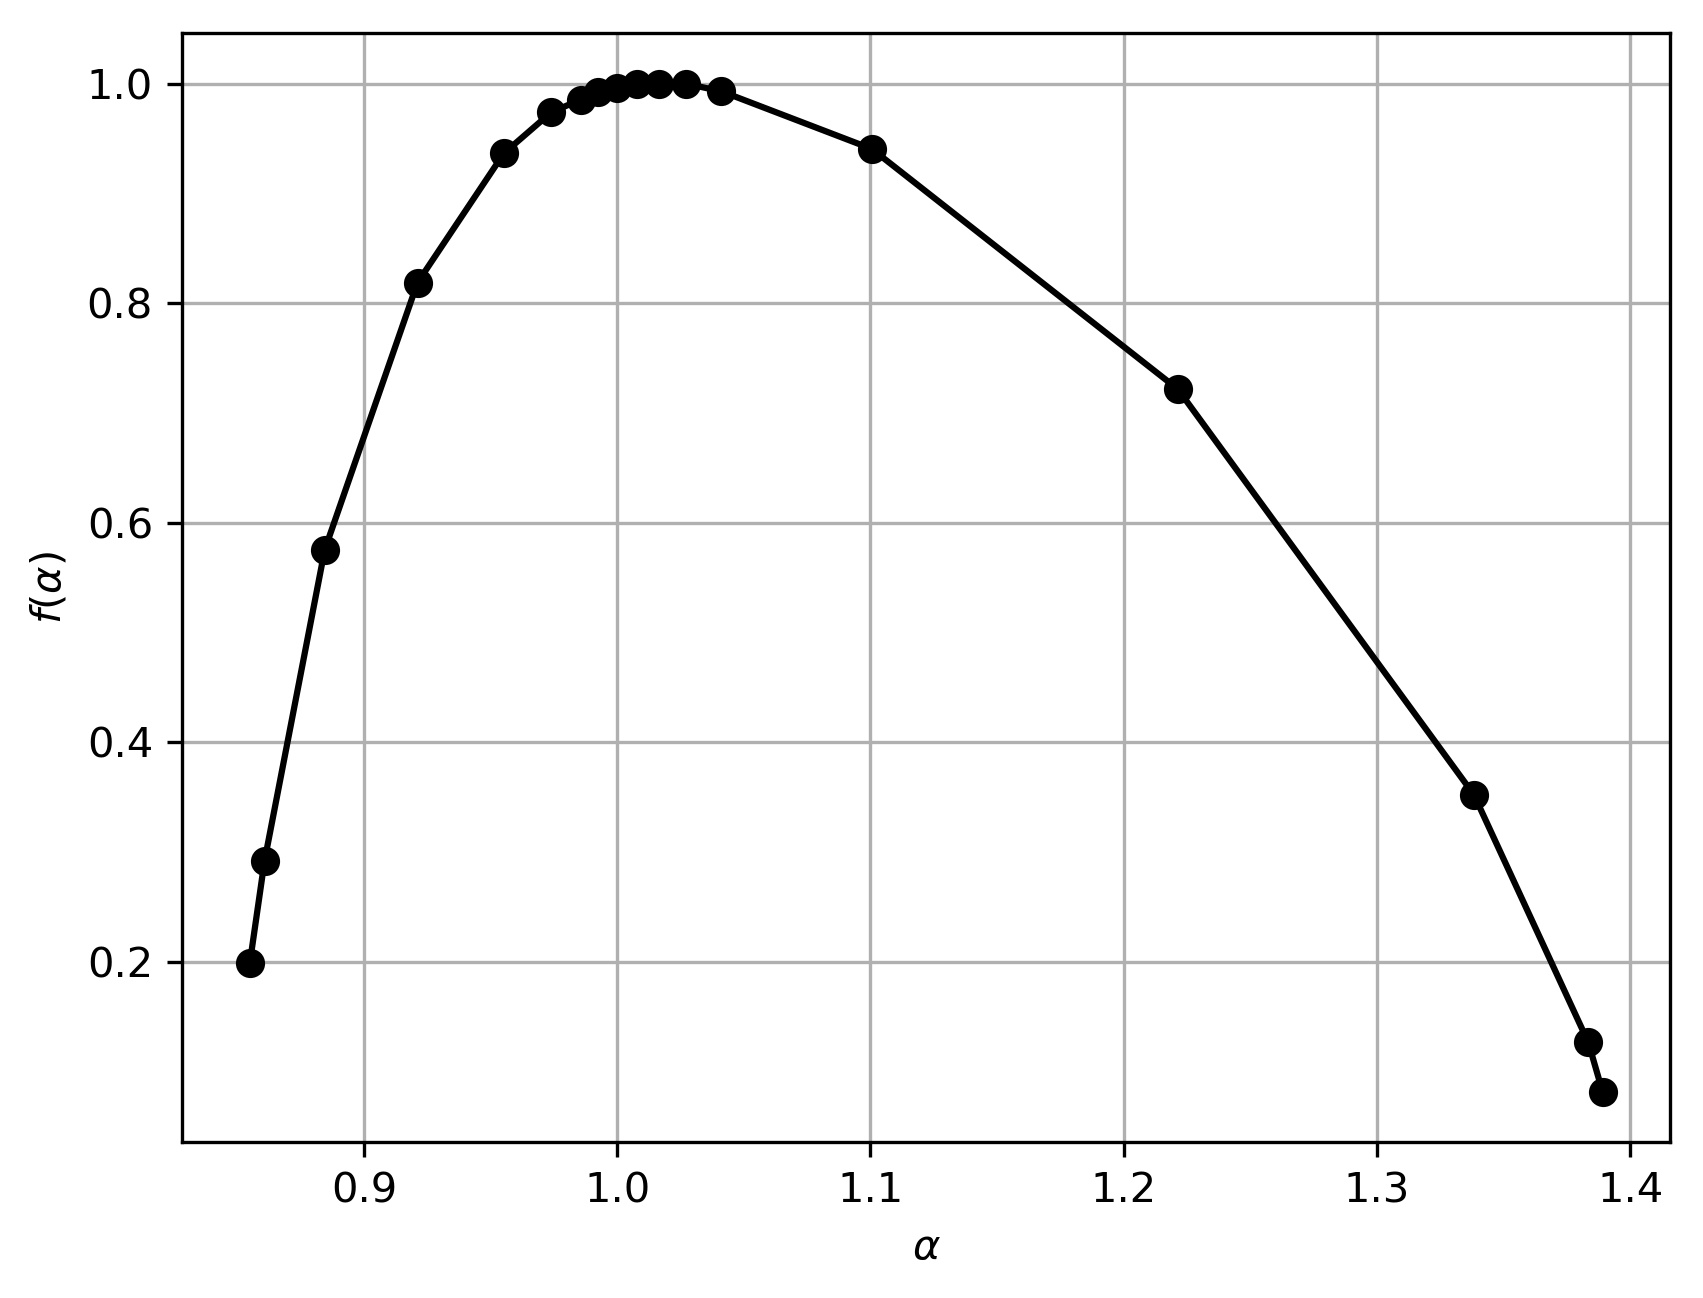
\includegraphics{Figuras/ex7/7_2/Exercicio7_2_grupo_noise_n_8192_mfdfa_4.jpg}}		
	\end{center}
	\vspace{-2mm}	% acrescentar o espaçamento vertical apropriado entre a borda inferior da figura e a legenda ou a fonte quando não há legenda (o valor pode ser negativo para subir)
	\legenda{Figura 7.2.4: Espectro de singularidade $f(\alpha)$ vs $\alpha$ do grupo noise com $n$ = 8192.}	% legenda - para deixar sem legenda usar comando \legenda{} (nunca deve-se comentar o comando \legenda)
	\label{ex6_fig1}
	%\FONTE{}	% fonte consultada (elemento obrigatório, mesmo que seja produção do próprio autor)
\end{figure}


%%%%%%%%%%%%%%%%%%%%%%%%%%%%%%%%%%% Analise extra %%%%%%%%%%%%%%
%\clearpage
\subsubsection*{Monofractalidade vs Multifractalidade}

Uma análise interessante é a comparação do espectro de singularidade entre dois grupos particulares da tabela \textit{Dataset\_signal}: chaosnoise e pmnoise. O espectro de singularidade para o mapeamento Logístico e para uma série exógena (Figura 7.2.5) são apresentados a seguir.

O valor de $\Delta \alpha$ = $\alpha_{max} - \alpha_{min}$ reflete a multifractalidade da série. Quanto maior o $\Delta \alpha$, maior a característica multifractal e complexidade da série, e a distribuição apresenta flutuações mais severas. Mapas caóticos como o mapeamento Logístico possuem uma faixa dinâmica estreita e apresentam monofractalidade, de modo que seu espectro de singularidade indica um valor de $\Delta \alpha$ relativamente pequeno: a curva em vermelho da Figura 7.2.5 não se extende nas duas extremidades (ela é monofractal-like). Por outro lado, a série exógena do pmodel apresenta multifractalidade, de forma que seu $\Delta \alpha$ é maior conforme evidenciado pelo espectro de singularidade.

\begin{figure}[ht!]
	%\caption{Série e histogramas.}
	\vspace{0mm}	% acrescentar o espaçamento vertical apropriado entre o título e a borda superior da figura
	\begin{center}
		\resizebox{16cm}{!}{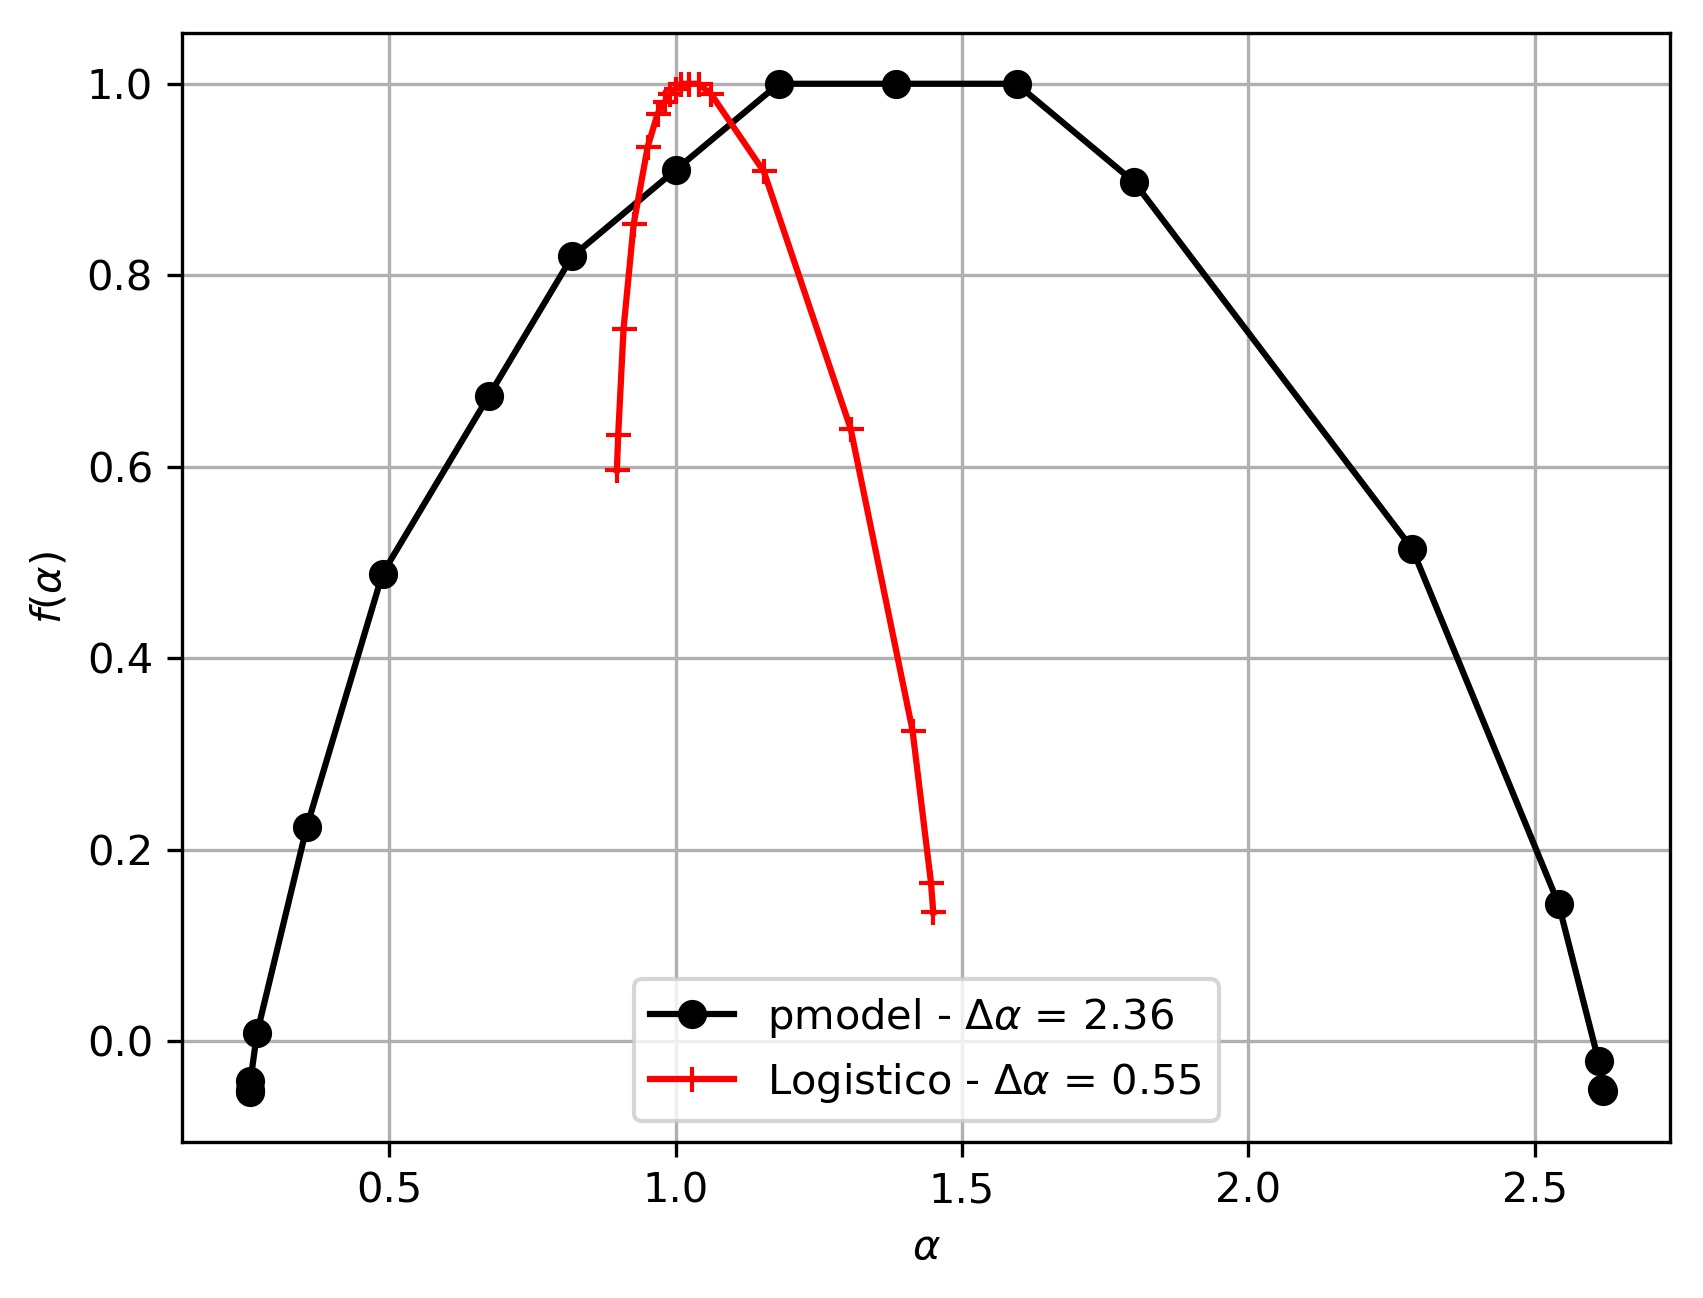
\includegraphics{Figuras/ex7/7_2/comp_mfdfa_4.jpg}}		
	\end{center}
	\vspace{-2mm}	% acrescentar o espaçamento vertical apropriado entre a borda inferior da figura e a legenda ou a fonte quando não há legenda (o valor pode ser negativo para subir)
	\legenda{Figura 7.2.5: Comparação entre o espectro de singularidade $f(\alpha)$ vs $\alpha$ do grupo pmnoise e do grupo chaosnoise. Série exógena do pmodel com $p$ = 0.18 e $\beta$ = 0.7 vs mapeamento Logístico com $\rho$ = 3.81.}	% legenda - para deixar sem legenda usar comando \legenda{} (nunca deve-se comentar o comando \legenda)
	\label{ex6_fig1}
	%\FONTE{}	% fonte consultada (elemento obrigatório, mesmo que seja produção do próprio autor)
\end{figure}

%\begin{figure}[ht!]
	%\caption{Série e histogramas.}
%	\vspace{-3mm}	% acrescentar o espaçamento vertical apropriado entre o título e a borda superior da figura
%	\begin{center}
%		\resizebox{12cm}{!}{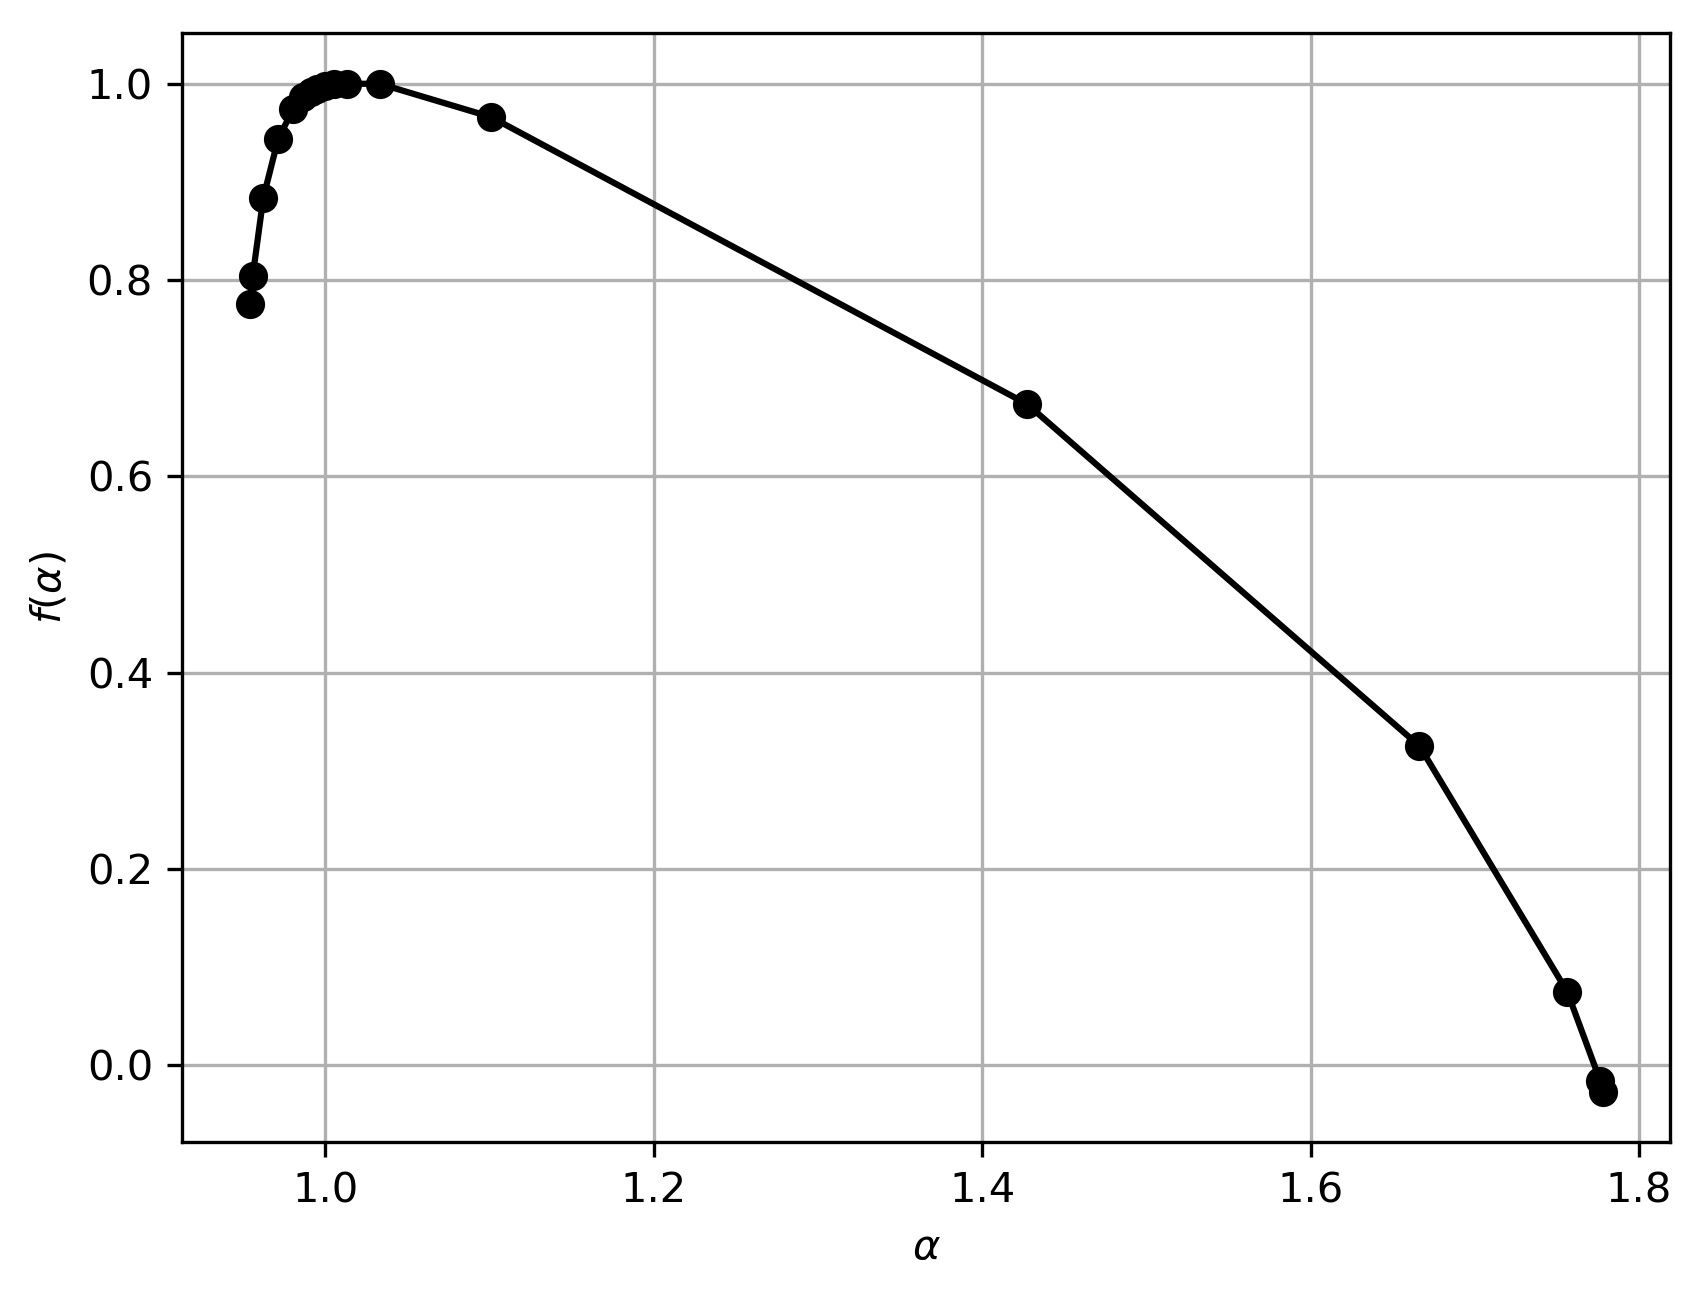
\includegraphics{Figuras/ex7/7_2/Exercicio7_2_Logistico_rho_3.81_mfdfa_4.jpg}}		
%	\end{center}
%	\vspace{-3mm}	% acrescentar o espaçamento vertical apropriado entre a borda inferior da figura e a legenda ou a fonte quando não há legenda (o valor pode ser negativo para subir)
%	\legenda{Figura 7.2.5: Espectro de singularidade $f(\alpha)$ vs $\alpha$ do grupo chaosnoise: mapeamento Logístico com $\rho$ = 3.81.}	% legenda - para deixar sem legenda usar comando \legenda{} (nunca deve-se comentar o comando \legenda)
%	\label{ex6_fig1}
	%\FONTE{}	% fonte consultada (elemento obrigatório, mesmo que seja produção do próprio autor)
%\end{figure}

%\begin{figure}[ht!]
	%\caption{Série e histogramas.}
%	\vspace{-3mm}	% acrescentar o espaçamento vertical apropriado entre o título e a borda superior da figura
%	\begin{center}
%		\resizebox{12cm}{!}{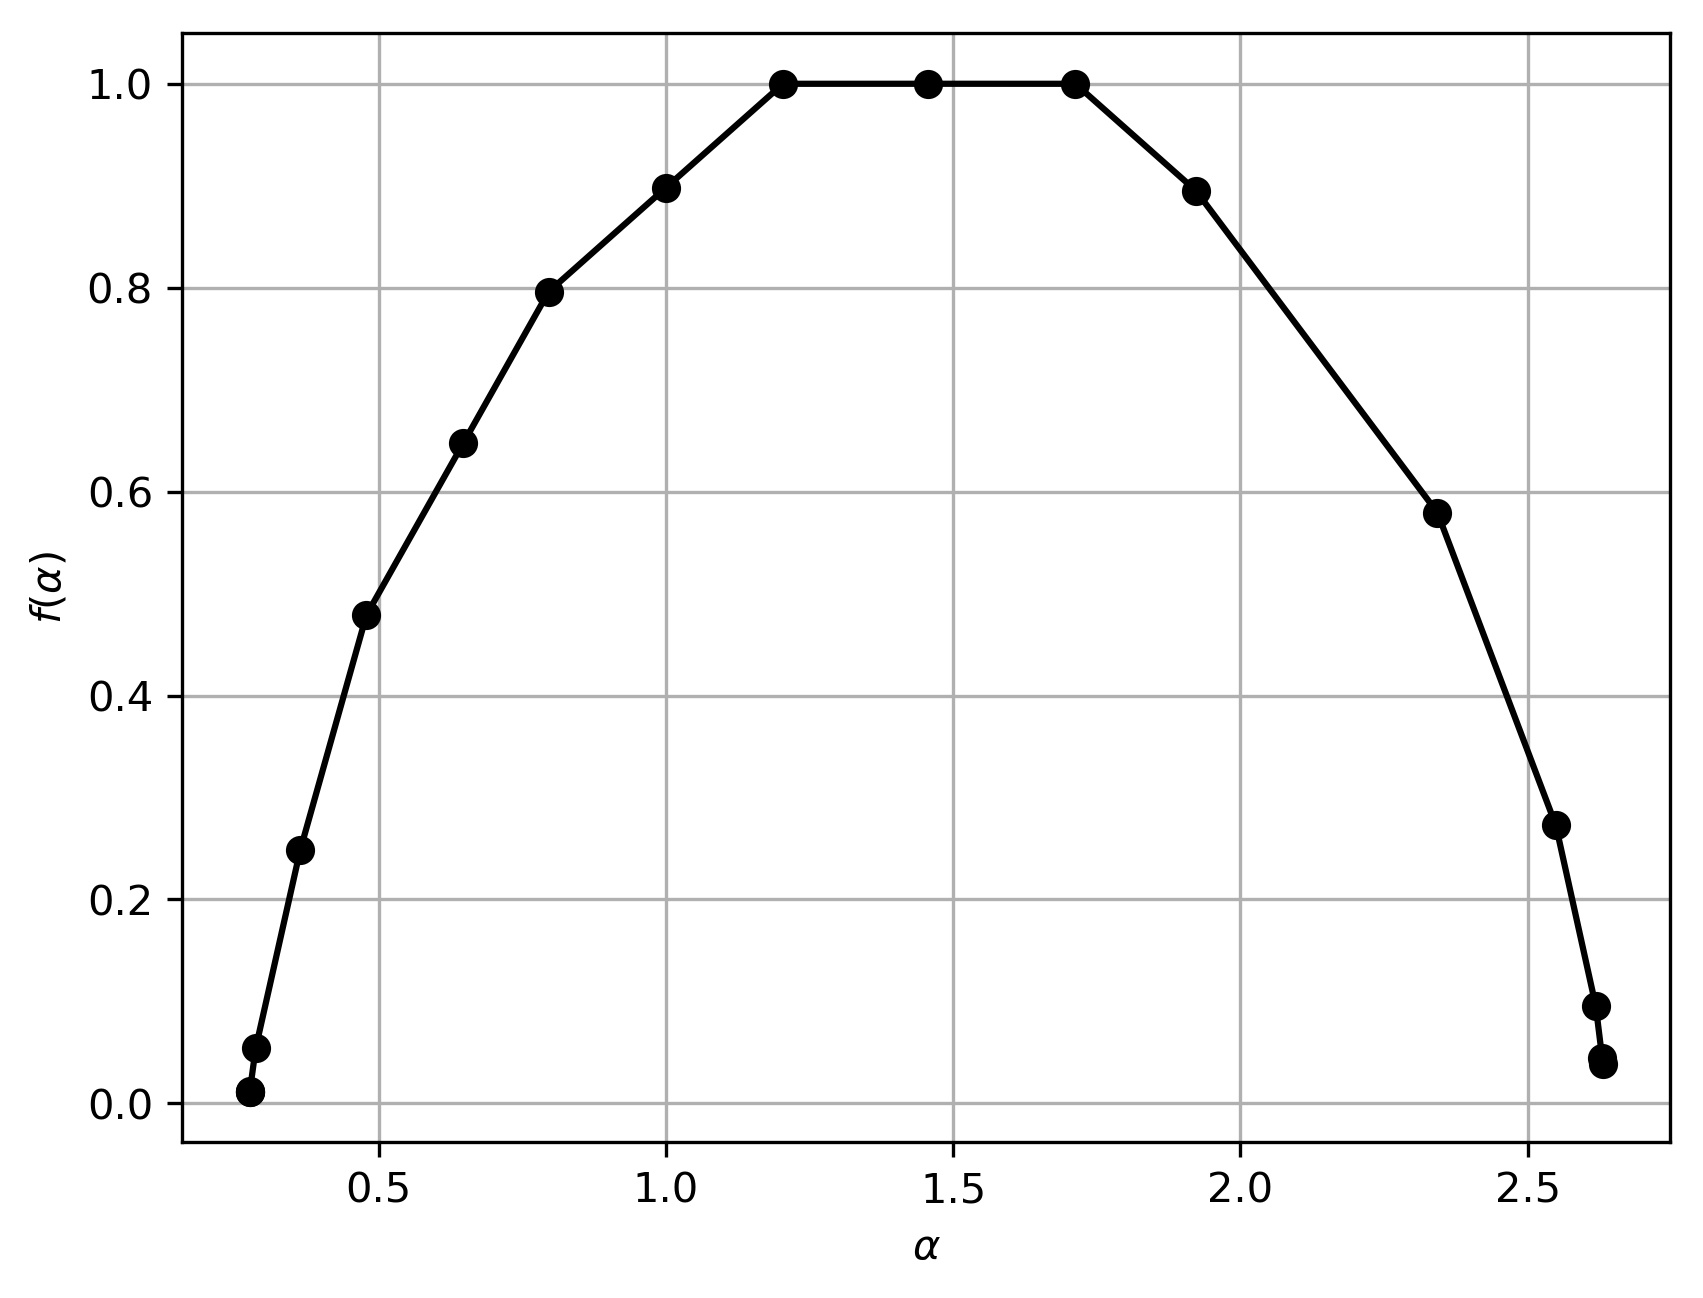
\includegraphics{Figuras/ex7/7_2/Exercicio7_2_grupo_pmnoise_p_0.18_mfdfa_4.jpg}}		
%	\end{center}
%	\vspace{-3mm}	% acrescentar o espaçamento vertical apropriado entre a borda inferior da figura e a legenda ou a fonte quando não há legenda (o valor pode ser negativo para subir)
%	\legenda{Figura 7.2.6: Espectro de singularidade $f(\alpha)$ vs $\alpha$ do grupo pmnoise: série exógena com $p$ = 0.18 e $\beta$ = 0.7.}	% legenda - para deixar sem legenda usar comando \legenda{} (nunca deve-se comentar o comando \legenda)
%	\label{ex6_fig1}
	%\FONTE{}	% fonte consultada (elemento obrigatório, mesmo que seja produção do próprio autor)
%\end{figure}


%%%%%%%%%%%%%%%%%%%%%%%%%%%%%%%%%%%  7.3 %%%%%%%%%%%%%%%%%%%%%%%%%%%%
\clearpage
\subsection*{7.3}
\addcontentsline{toc}{section}{\protect\numberline{} 7.3}%

Os resultados deste exercício estão presentes na pasta \textbf{7.3}. Abaixo o plot do melhor número de clusters determinado pelo méotodo do cotovelo. O algoritmo utilizado foi o kmeans\_2D\_group\_flags.py, que agrupou cada país em seu respectivo cluster em arquivos .csv (identificados pelo centróide do grupo).

\begin{figure}[ht!]
	%\caption{Série e histogramas.}
	\vspace{0mm}	% acrescentar o espaçamento vertical apropriado entre o título e a borda superior da figura
	\begin{center}
		\resizebox{15cm}{!}{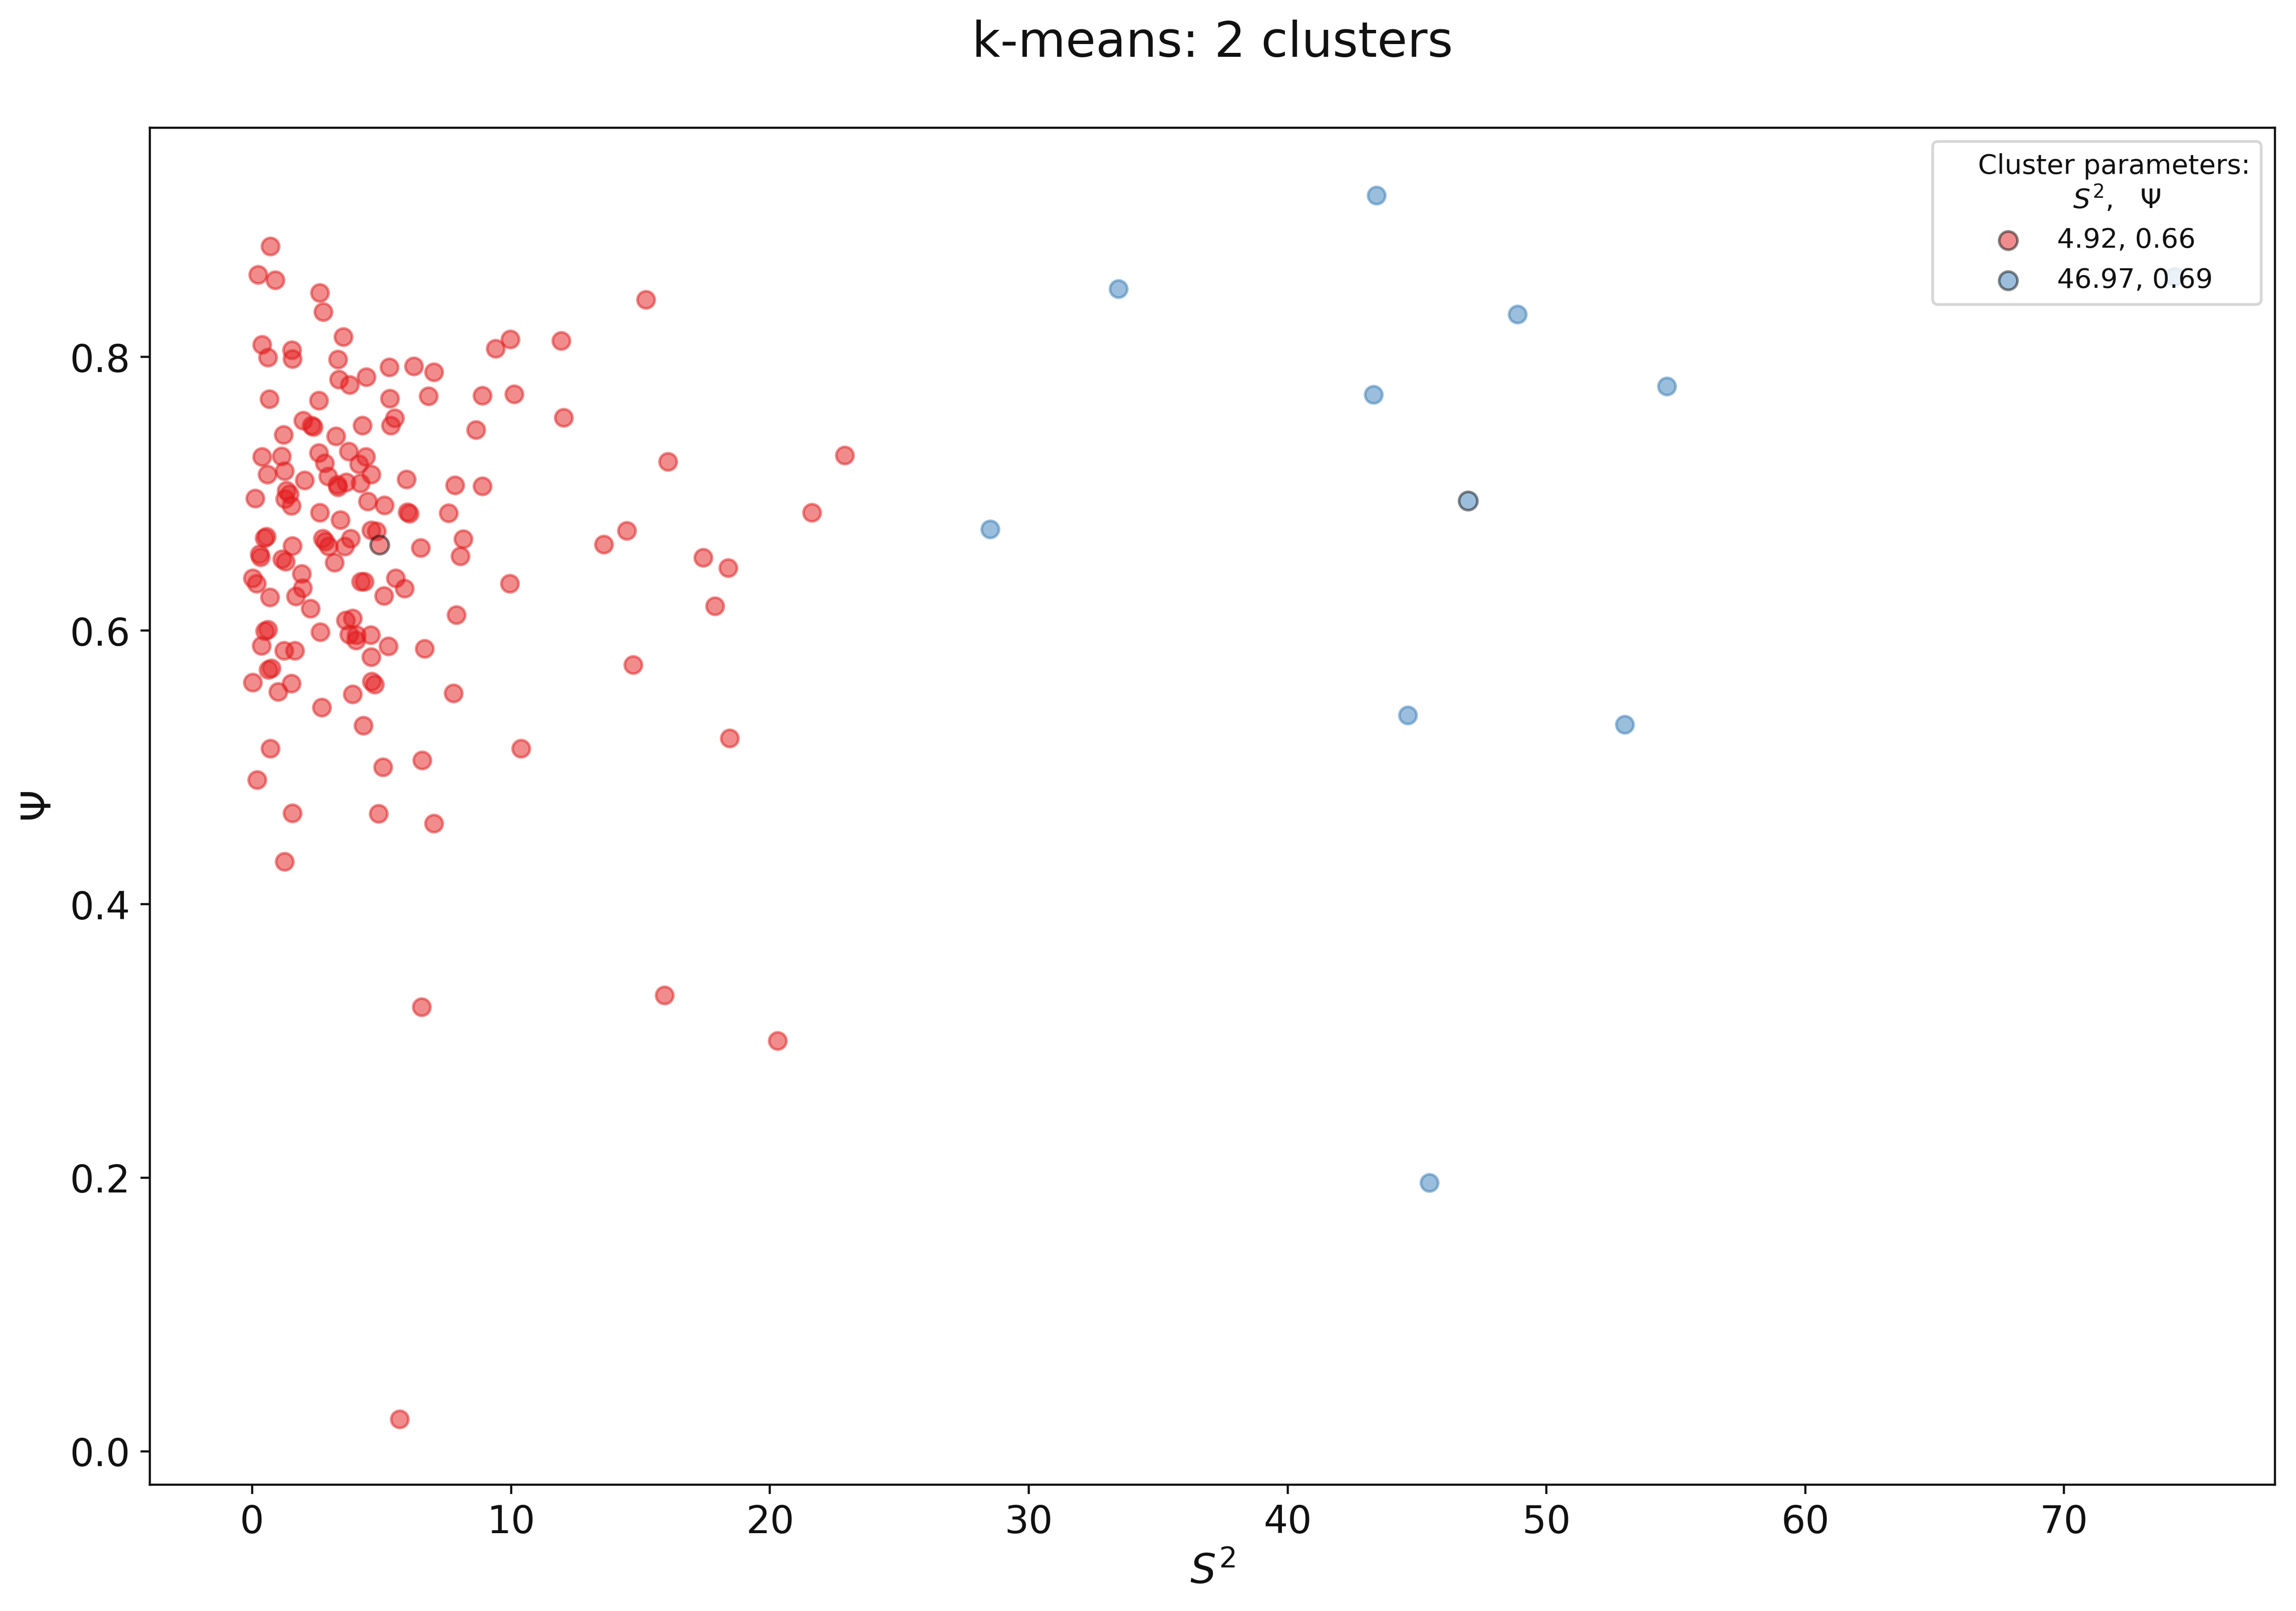
\includegraphics{Figuras/ex7/7_3/Exercicio7_3_cluster_2.jpg}}		
	\end{center}
	\vspace{-2mm}	% acrescentar o espaçamento vertical apropriado entre a borda inferior da figura e a legenda ou a fonte quando não há legenda (o valor pode ser negativo para subir)
	\legenda{Figura 7.3.1: Resultado do agrupamento do número de casos diários de Covid19 para todos os países no espaço S$^{2}$ x $\Psi$. O valor $n\_c$ = 2 obteve a melhor performance.}	% legenda - para deixar sem legenda usar comando \legenda{} (nunca deve-se comentar o comando \legenda)
	\label{ex6_fig1}
	%\FONTE{}	% fonte consultada (elemento obrigatório, mesmo que seja produção do próprio autor)
\end{figure}

Neste exercício, os grupos de países se encontram nos seguintes arquivos: \textit{Exercicio7\_3\_cluster\_0\_x\_3.58\_y\_0.62\_flags.csv} (cluster vemelho) e \textit{Exercicio7\_3\_cluster\_1\_x\_36.38\_y\_0.62\_flags.csv} (cluster azul).